% ---------- Metadata ----------
\title[Aula 6]{Aula 6 - Título da Aula}
\author[Marcato]{Professor: André L. Marcato}
\institute[UFJF]{Universidade Federal de Juiz de Fora \\ Engenharia Elétrica — Robótica e Automação Industrial}

% ---------- Title ----------
\begin{frame}
  \titlepage
\end{frame}

% ---------- Overview ----------
\begin{frame}{Roteiro}
\tableofcontents
\end{frame}

% ---------- Conteúdo ----------

% ---------- Conteúdo Aula 6 ----------
\section{Conceitos de Actions}

% --- Slide: Definição e Diferenças ---
\begin{frame}[fragile]{\href{https://docs.ros.org/en/humble/Tutorials/Beginner-CLI-Tools/Understanding-ROS2-Actions/Understanding-ROS2-Actions.html}{\uline{ROS 2 — Actions}}}
  \begin{itemize}
    \item \textbf{Actions}: Comunicação para tarefas de \textbf{longa duração}.
    \item Diferente de Services (síncrono/rápido) e Topics (streaming contínuo).
    \item Composta por três partes:
      \begin{itemize}
        \item \textbf{Goal}: O pedido enviado pelo cliente (início).
        \item \textbf{Feedback}: Dados periódicos sobre o progresso (durante).
        \item \textbf{Result}: O dado final após a conclusão (fim).
      \end{itemize}
    \item \textbf{Características}: Pode ser cancelada, preemptada e rejeitada.
  \end{itemize}
\end{frame}

% --- Slide: Arquitetura ---
\begin{frame}{Arquitetura de Actions}
  \centering
  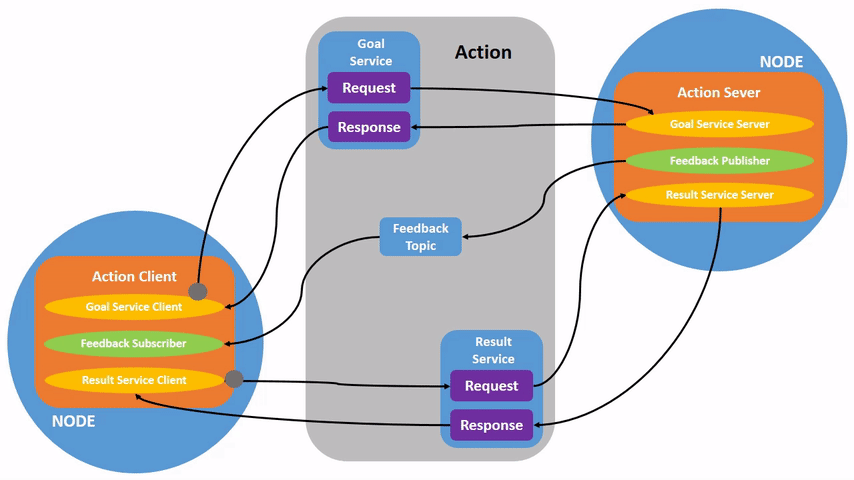
\includegraphics[width=0.9\textwidth]{aula6/images/code_action_server.png}
\end{frame}

% --- Slide: Estrutura .action ---
\begin{frame}[fragile]{Interface .action}
  \begin{itemize}
    \item Definida em arquivos \texttt{.action}.
    \item Separada por \textbf{três traços} (\texttt{---}).
  \end{itemize}

  \begin{center}
  
\includegraphics[width=0.7\textwidth]{code_fibonacci_action.png}
  \end{center}
\end{frame}

% --- Slide: Comandos CLI ---
\begin{frame}[fragile]{Actions — Comandos úteis (CLI)}
  \textbf{Inspeção}
\begin{lstlisting}[style=bashstyle]
# Listar actions
$ ros2 action list -t
# Ver estrutura (Goal/Result/Feed)
$ ros2 interface show action_tutorials_interfaces/action/Fibonacci
# Informações do nó
$ ros2 action info /fibonacci
\end{lstlisting}

  \vspace{0.6em}

  \textbf{Enviar Goal}
\begin{lstlisting}[style=bashstyle]
# Enviar goal com feedback
$ ros2 action send_goal \
  /fibonacci \
  action_tutorials_interfaces/action/Fibonacci \
  "{order: 5}" --feedback
\end{lstlisting}
\end{frame}

\section{Implementação em Python}

% --- Slide: Servidor (Python) ---
\begin{frame}[fragile]{Action Server (Python) — \texttt{Fibonacci}}
  \begin{center}
  
\includegraphics[width=0.65\textwidth]{code_fibonacci_action_server.png}
  \end{center}
\end{frame}

% --- Slide: Cliente (Python) ---
\begin{frame}[fragile]{Action Client (Python) — \texttt{Fibonacci}}
  \begin{center}
  
\includegraphics[width=0.75\textwidth]{code_fibonacci_action_client.png}
  \end{center}
\end{frame}


\section{Prática: Interfaces}

% --- Slide: Criando o pacote de Interfaces ---
\begin{frame}[fragile]{Prática — Criar Interface Action}
  \begin{itemize}
    \item Interfaces devem ficar em pacotes dedicados (CMake).
  \end{itemize}

\begin{lstlisting}[style=bashstyle]
$ cd ~/ros2_ws/src
$ ros2 pkg create action_tutorials_interfaces
$ cd action_tutorials_interfaces
$ mkdir action
# Crie action/Fibonacci.action aqui
\end{lstlisting}

\textbf{CMakeLists.txt}:
  \begin{center}
  
\includegraphics[width=0.7\textwidth]{code_cmake_action.png}
  \end{center}
\end{frame}


\section{Prática: Server \& Client}

% --- Slide: Pacote Python ---
\begin{frame}[fragile]{Prática — Pacote Python e Dependências}
  \begin{itemize}
    \item Crie o pacote e defina as dependências.
  \end{itemize}
\begin{lstlisting}[style=bashstyle]
$ cd ~/ros2_ws/src
$ ros2 pkg create --build-type ament_python action_tutorials_py \
  --dependencies rclpy action_tutorials_interfaces
\end{lstlisting}

  \begin{itemize}
    \item Implemente os códigos Python (Server e Client).
    \item Adicione entry points no \texttt{setup.py}.
  \end{itemize}

  \begin{center}
  
\includegraphics[width=0.75\textwidth]{code_setup_entry_points.png}
  \end{center}
\end{frame}

% --- Slide: Execução e Teste ---
\begin{frame}[fragile]{Prática — Execução e Teste}
\textbf{Terminal 1 (Server):}
\begin{lstlisting}[style=bashstyle]
$ colcon build --symlink-install
$ source install/setup.bash
$ ros2 run action_tutorials_py fibonacci_action_server
\end{lstlisting}

\vspace{0.5em}
\textbf{Terminal 2 (Teste via CLI):}
\begin{lstlisting}[style=bashstyle]
$ ros2 action send_goal /fibonacci \
  action_tutorials_interfaces/action/Fibonacci "{order: 10}"
\end{lstlisting}

\vspace{0.5em}
\textbf{Terminal 3 (Teste via Client Node):}
\begin{lstlisting}[style=bashstyle]
$ ros2 run action_tutorials_py fibonacci_action_client
\end{lstlisting}
\end{frame}

% --- Slide: Exercício Proposto ---
\begin{frame}[fragile]{Exercício Proposto}
  \begin{block}{Objetivo: Robô Rotativo}
    Criar uma Action que simula um robô girando até um ângulo.
  \end{block}
  \begin{itemize}
    \item \textbf{Goal}: \texttt{float32 target\_angle}
    \item \textbf{Feedback}: \texttt{float32 current\_angle}
    \item \textbf{Result}: \texttt{string message} ("Alvo atingido")
    \item \textbf{Lógica}: O servidor deve incrementar o ângulo em loop (use \texttt{time.sleep(0.5)}) publicando feedback até chegar no alvo.
  \end{itemize}
\end{frame}
